\chapter{Cenário Atual da Manutenção de Equipamentos na UnB}
\label{man-unb}

Esse capítulo mostra o cenário atual da manutenção de equipamentos da Universidade de Brasília, descrevendo a Diretoria de Manutenção de Equipamentos, o Sistema de Patrimônio (SIPAT), responsável pelo inventariado dos bens da universidade e que contém algumas funcionalidades relacionadas a manutenção. E também descreverá o processo atual seguido pela DIMEQ para realização da manutenção.

%--------------------------------------------------------------------------------------------------%

\section{Diretoria de Manutenção de Equipamentos (DIMEQ)}

Em 30 de outubro de 1987, pelo ato da reitoria nº 550, foi criada Diretoria de Manutenção de Equipamentos - DIMEQ, anteriormente denominado Centro de Manutenção de Equipamentos Científicos – CME da Fundação Universidade de Brasília, garantido a ela, desde então, o tratamento autônomo e descentralizado sob o aspecto orçamentário, financeiro, administrativo e gerencial \cite{dimeq}.

Por este ato da reitoria foi atribuída a DIMEQ à responsabilidade de promover, com qualidade, a manutenção e o reparo nos equipamentos da Universidade, introduzindo novos conceitos metodológicos e técnicos para que sejam reduzidas as paradas de funcionamento desses equipamentos; visando a redução de custos, a satisfação do usuário e a viabilização das atividades de ensino e pesquisa.

Na estrutura organizacional da DIMEQ estão compreendidas quatro seções especializadas, a saber, Seção de Apoio a Logística, Seção de Eletrônica e Informática, Seção de Eletromecânica e Seção Mecânica. Esta configuração se fez necessária, em suma, pelos tipos de equipamentos que a Universidade possui, os quais precisam ser agrupados, pois cada tipo de equipamento necessita de uma mão de obra especifica, bem como instrumentos e ferramentas para fins de manutenção. São eles, equipamentos eletrônicos, de informática, eletromecânicos, eletrotécnicos, ópticos e de mecânica fina, e os mecânicos que, por sua vez, se dividem de refrigeração e de mecânica geral.

Os serviços prestados pela DIMEQ devem atender uma comunidade acadêmica bastante ampla, o que faz do processo de manutenção permanente um grande desafio, sendo composta, segundo informações do Anuário Estatístico da UnB 2015 \cite{anuario2015}), de 2.695 professores, 2.623 técnicos-administrativos e 36.372 alunos regulares e 7.576 de pós-graduação. Constituída por 26 institutos e faculdades e 21 centros de pesquisa especializados, oferecendo 109 cursos de graduação, e 147 cursos de pós-graduação stricto sensu e 22 especializações lato sensu. Os cursos estão divididos em quatro campi espalhados pelo Distrito Federal: Darcy Ribeiro (Plano Piloto), Planaltina, Ceilândia e Gama, possuindo diversos órgãos de apoio como o Hospital Universitário, a Biblioteca Central, o Hospital veterinário e a Fazenda Água Limpa.

Somado a grande comunidade acadêmica que a DIMEQ precisa atender, encontra-se o diversificado parque científico que a Universidade de Brasília possui. Esta diversificação, a complexidade e quantidade de equipamentos demandam, segundo \cite{limacastilho2006} um elevado estoque de peças de reposição, espaço físico, qualificação permanente dos técnicos, meios de transporte específicos e, sobretudo, um sistema de gerenciamento e comunicação que esteja em constante evolução, pronto a atender as necessidades emergentes. Há ainda, diversos equipamentos importados que requerem na maioria das vezes, serviços especializados.

Ao visualizar os números da Universidade, pode se ter uma noção do desafio que é gerenciar as manutenções dos equipamentos, ainda mais quando se estuda o crescimento da população Universitária da UNB de 2006 a 2014, conforme demonstra os Figura~\ref{grafico_dimeq1} e Figura~\ref{grafico_dimeq2}, retirados do anuário estatístico da Universidades de 2011 e 2015, respectivamente. Eles revelam que nestes 8 anos a população universitária cresceu 56,95\% aproximadamente.

\graphicspath{{figuras/}}
\begin{figure}[H]
\centering
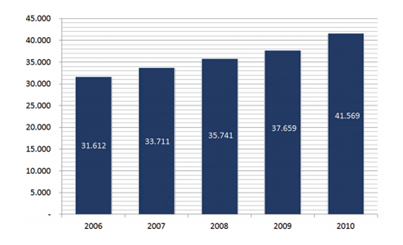
\includegraphics[width=0.9\textwidth]{grafico_dimeq1}
\caption{Evolução da população universitária da UnB, 2006 a 2010. \textbf{Fonte: Anuário estatístico da Universidade de Brasília, 2011.}}
\label{grafico_dimeq1}
\end{figure}


\graphicspath{{figuras/}}
\begin{figure}[H]
\centering
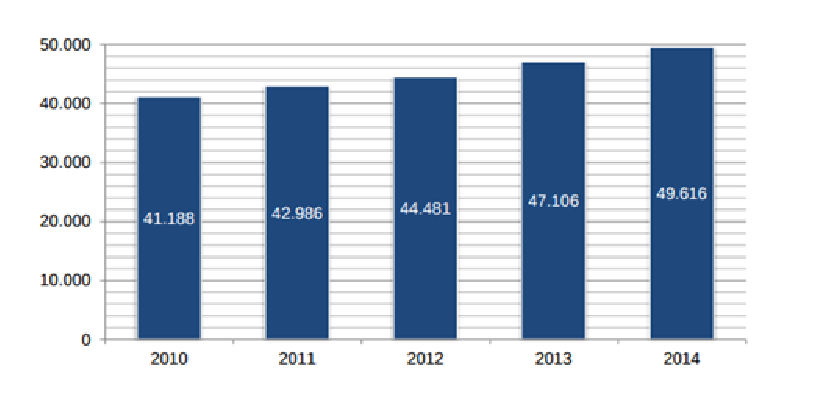
\includegraphics[width=0.9\textwidth]{grafico_dimeq2.eps}
\caption{Evolução da população universitária da UnB, de 2010 a 2014. \textbf{Fonte: Novo anuário estatístico da Universidade de Brasília, 2015.}}
\label{grafico_dimeq2}
\end{figure}

Todo esse crescimento deve ser levado em conta ao se analisar o serviço de Manutenção oferecido pela DIMEQ, pois sua conseqüência é um enorme descompasso entre a quantidade de adquiridos e os recursos aplicados na preservação desse patrimônio. Além de que, conforme relata \cite{limacastilho2006} ao se adquirir esses equipamentos \lq\lq patrimônios\rq\rq a DIMEQ não foi ouvida cometendo assim um erro conceitual grave para gestão da Manutenção, como já foi relatado no capítulo de Manutenção do presente trabalho.
	
O gerenciamento da manutenção do parque cientifico da UnB é informatizado, permitindo a todos os usuários solicitar e acompanhar reparos nos equipamentos ou a programação de manutenção preventiva de todos os equipamentos cadastrados no Sistema de Informações Patrimoniais (SIPAT), sejam eles da UnB ou de outras instituições. 
	
Para facilitar o gerenciamento da manutenção, a DIMEQ utiliza informações básicas, a partir do ingresso do equipamento e dos registros das ocorrências, envolvendo fornecedores e a própria equipe da DIMEQ, mesmo que esses equipamentos sejam oriundos de convênio e comodatos.
	
O público atendido pela DIMEQ é denominado usuário, e a informação que mais os interessa é o tempo que o equipamento ficará indisponível durante a manutenção, sendo chamado de tempo total de manutenção caracterizado pelo tempo total que o equipamento fica indisponível para a utilização, ou seja, o tempo decorrente entre a solicitação e a conclusão do serviço. O qual é um indicador monitorado e visível aos usuários das manutenções providas pelas DIMEQ.

Todavia, vê-se que apesar da Diretoria de Manutenção de Equipamento da Universidade de Brasília se esforçar para oferecer aos usuários um bom serviço, não possui controles estatísticos e probabilísticos sobre os ciclos de vida útil dos Equipamentos, implantando assim somente uma política de manutenções corretivas e emergenciais. Não possuindo indicadores de custo efetivos que embasem decisões relacionadas as manutenções. 

%---------------------------------------------------------------------------------------------------------%

\section{Sistema de Patrimônio - SIPAT}

O Sistema de Patrimônio da Unb, SIPAT, responsável pela Gestão do patrimônio mobiliário da UnB e das manutenções de
equipamentos do DIMEQ/PRC, foi desenvolvido pelo Centro de Processamento de Dados - CPD. Sua primeira versão foi liberada em 1964, sendo desenvolvido em \textit{Cobol}. Com o famoso bug do milênio, que iria ocorrer no ano 2000, em 1999 o código foi refatorado e reescrito para \textit{visual basic, vb6}, escolhido pelo suporte que seria dado pela Microsoft. A transição dos sistemas levou 8 meses, os grandes e de 4 a 5 meses nos pequenos.

Segundo um técnico do CPD, que descreveu o sistema e explicou como ele funcionava e como foi desenvolvido, o SIPAT é mais utilizado pelo setor de Patrimônio, sendo acoplado ao sistema de pessoal, para verificar a carga patrimonial. Possui também algumas funcionalidades voltadas para manutenção, que são utilizadas pela DIMEQ.

A versão atualmente utilizada, como já escrito, foi desenvolvida em virtual basic e está sendo utilizada desde o ano 2000, após uma massiva refatoração feito pelo CPD nos sistemas da universidade. O SIPAT trabalha em 3 camadas: \textbf{Servidor de Aplicação}, \textbf{Servidor de Banco de Dados} e \textbf{Sistema Cliente}. Ele é instalado e utilizado pela Intranet da Unb. Sua instalação tem que ser solicitada pelo usuário ao CPD.

Quanto a documentação do sistema, na reunião realizada com dois técnicos do CPD, em dezembro de 2016, foi explicado que eles seguem a metodologia de desenvolvimento RUP e estão estudando passar para Ágil, e portanto possui alguns documentos, todos defasados, e que as funcionalidades foram apenas descritas, na primeira versão, mais eles não possuem nenhum rastreio dos requisitos.

A Tabela~\ref{sipat1}, mostra as funcionalidades do SIPAT voltadas para o PAT, setor de Patrimônio, e a Tabela~\ref{sipat2}, mostra as funcionalidades que são mais utilizadas pela DIMEQ, relativas a manutenção de equipamentos. As dados foram retiradas do Manual do Usuário do SIPAT. 


\begin{table}[H]
\centering
\caption{Principais Funcionalidades do SIPAT. Fonte: Autor.}
\label{sipat1}
\begin{tabular}{ | p{15cm} |}
\hline
	Registro de Material Permanente e Tombamento. \\ \hline
	Solicitação de Instalação ou Reparo. \\ \hline
	Solicitação de inspeção para redistribuição ou baixa. \\ \hline
	Cadastro de Agente Patrimonial. \\ \hline
	Consulta de dados básicos dos bens, locais e agentes cadastrados. \\ \hline
	Consulta de  andamento da solicitação de reparo. \\ \hline
	Consulta de laudo de Inspeção. \\ \hline
	Consulta do histórico da movimentação dos bens. \\ \hline
	Relatório de Termo de Transferência , Relação de Carga Patrimonial por Agente \\ \hline
	Relatório de Inventários por agente patrimonial \\ \hline
	Relatpórios de bens que estão em manutenção, Das solicitações de manutenção, bens alocados na unidade com valores unitários, total e quantitativo, classificados pelas contas do SIAFI e outros. \\ \hline
\end{tabular}
\end{table}

\begin{table}[H]
\centering
\caption{Funcionalidades voltadas para Manutenção. Fonte: Autor.}
\label{sipat2}
\begin{tabular}{ | p{15cm} |}
\hline
	SOLICITAÇÃO DE REPARO DE EQUIPAMENTO. \\ \hline
	ANDAMENTO DA MANUTENÇÃO/REPARO. \\ \hline
	SOLICITAÇÃO DE INSPEÇÃO PARA BAIXA OU REDISTRIBUIÇÃO. \\ \hline
	LAUDO DE VISTORIA.\\ \hline
\end{tabular}
\end{table}



%---------------------------------------------------------------------------------------------------------%

\section{Processo de Manutenção da DIMEQ}

\textbf{Processo e Modelagem de Processo.}

Business Process Modeling Notation (BPMN), é uma notação para modelar processos de negócios com intuito de facilitar o entendimento do processo. Antes de falar sobre a notação, é bom entender o que é um processo e porque modelá-lo facilita na sua visualização e entendimento. Segundo Hammer e Champy \cite{hammer1994reengenharia},\lq\lq um processo é um grupo de atividades realizadas numa sequência lógica com o objetivo de produzir um bem ou um serviço que tem valor para um grupo específico de clientes\rq\rq e Harrington \cite{harrington1993aperfeiccoando} diz, \lq\lq processo é qualquer atividade que recebe uma entrada (input), agrega-lhe valor e gera uma saída (output) para um cliente interno ou externo\rq\rq. Diante desses conceitos pode-se entender processo como atividades que são executadas sequencialmente, que tem entradas e saídas e geram ao final valor ao cliente.

Então, por que modelar um processo? O principal motivo de modelar um processo é facilitar a sua compreensão, assim como a UML tem diversos diagramas para o paradigma orientado a objetos, BPMN tem processos de negócio. A notação foi criada por Business Process Management Initiative (BPMI) e atualmente é mantida pelo Object Management Group, buscando padronizar essa representação gráfica.

Alguns dos elementos presentes na notação são descritos em Figura~\ref{table-processo}:


\graphicspath{{figuras/}}
\begin{figure}[H]
\centering
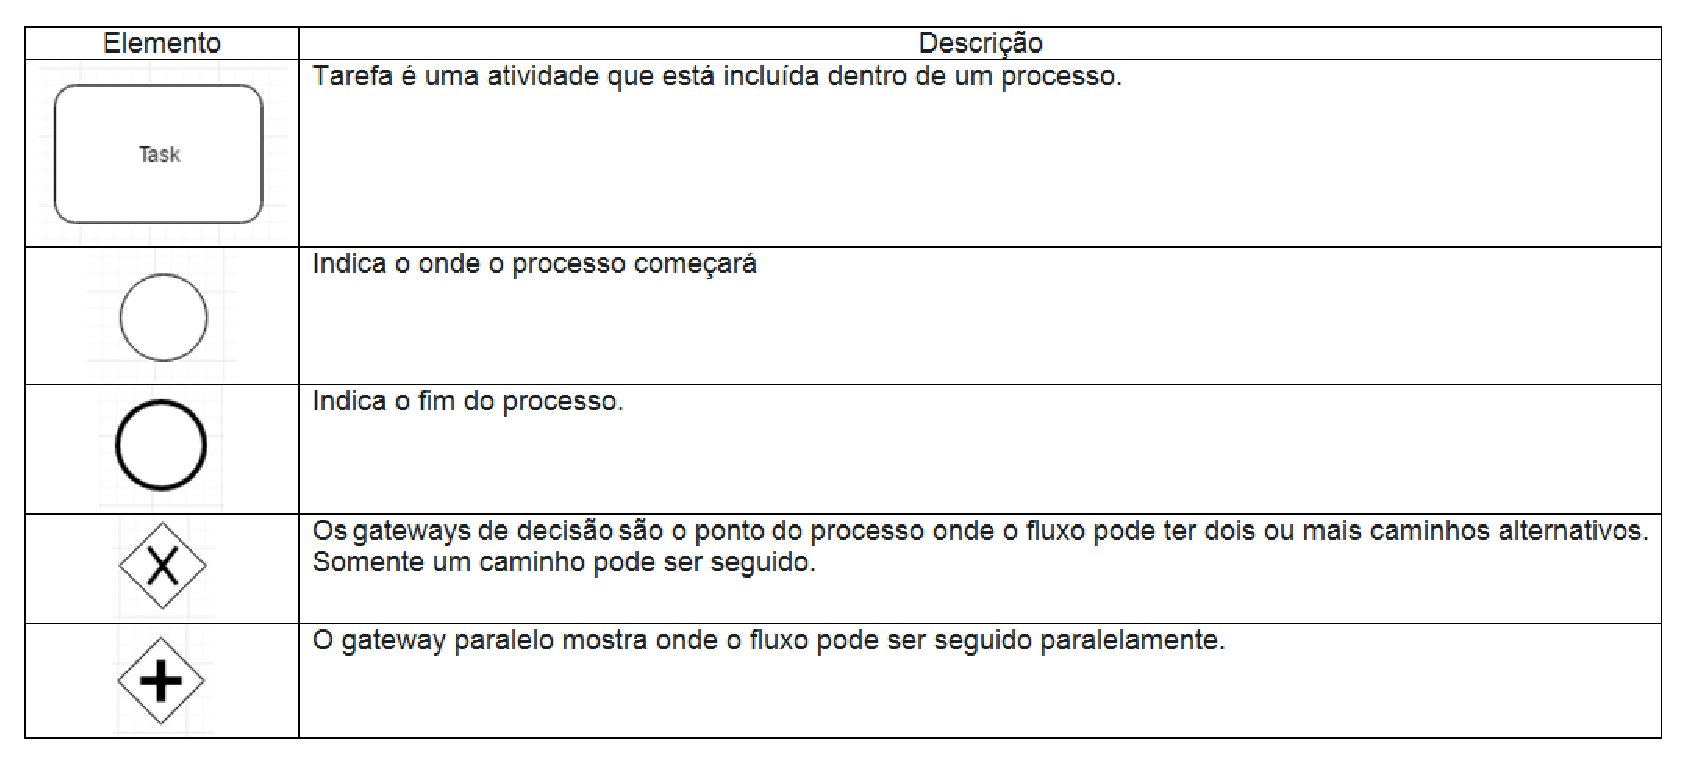
\includegraphics[width=1.0 \textwidth]{tabela-processo}
\caption{Descrição dos elementos do BPMN. \textbf{Adaptado de: Legenda BPMN.}}
\label{table-processo}
\end{figure}

%-------------------------------------------------------------------------------------------------%

\subsection{Explicação do Processo AS IS}
\label{processo-as-is}

O chamado processo AS IS, notação utilizada para descrever o processo atual, seguido pela Diretoria de Manutenção de Equipamentos da UnB, tem por objetivo reparar equipamentos e sugerir sua substituição caso seja necessário, como é visto na Figura~\ref{processo-as-is}.

Esse processo é iniciado pelo usuário que deseja abrir uma ordem de serviço, o qual é feito pelo SIPAT, Sistema Patrimonial. A Dimeq recebe a ordem de serviço também pelo sistema, imprimi e envia um técnico ao local designado para avaliar a situação do equipamento, se for possível reparar o equipamento no local, o técnico o faz, se não o equipamento é recolhido. Existe então outra bifurcação no processo relativa a existência de peças necessárias para o conserto do equipamento. Se eles tiverem as peças, o equipamento é reparado e devolvido ao usuário, senão é feita uma lista com as peças necessárias para que elas possam ser compradas. Após isso o equipamento é devolvido ao usuário e o responsável pelo reparo da a baixa do serviço pelo sistema.

A anotação no processo refere-se a uma regra definida no documento \textbf{Normas de Registro e Controle de Bens Patrimoniais Móveis da FUB}, de setembro de 2004, que diz no capítulo VIII,  art. 47, inciso II, parágrafo primeiro, \lq\lq Para os equipamentos que se encontrarem em reparo no CME, o Centro de Custo interessado poderá diligenciar ou indicar alternativas que viabilizem a sua recuperação, desde que o custo dos serviços não ultrapasse o limite de 50\% (cinqüenta por cento) do seu valor de mercado, de acordo com a Instrução Normativa SEDAP n. 205/1988. \rq\rq

\lq\lq As Normas de Registro e Controle dos Bens Patrimoniais Móveis, integrantes do Sistema de Gestão do Patrimônio Mobiliário da FUB (SIPAT), têm por finalidade estabelecer normas e procedimentos para regulamentar as atividades relativas ao tombamento, registro, controle, movimentação, baixa e inventário de bens móveis, incluindo os bens culturais, adquiridos pela Instituição, assim como à incorporação ao patrimônio da Fundação Universidade de Brasília dos bens e equipamentos provenientes de doações.\rq\rq (Normas de Registro e Controle dos Bens Patrimoniais Móveis, 2004).

O intuito do documento é juntar em um único lugar todas as normas internas que tratam da gestão do patrimônio da FUB (Fundação Universidade de Brasília), considerando os equipamentos, os materiais permanentes e os bens culturais e o seu devido valor para a instituição.

\begin{landscape}
\graphicspath{{figuras/}}
\begin{figure}[H]
\centering
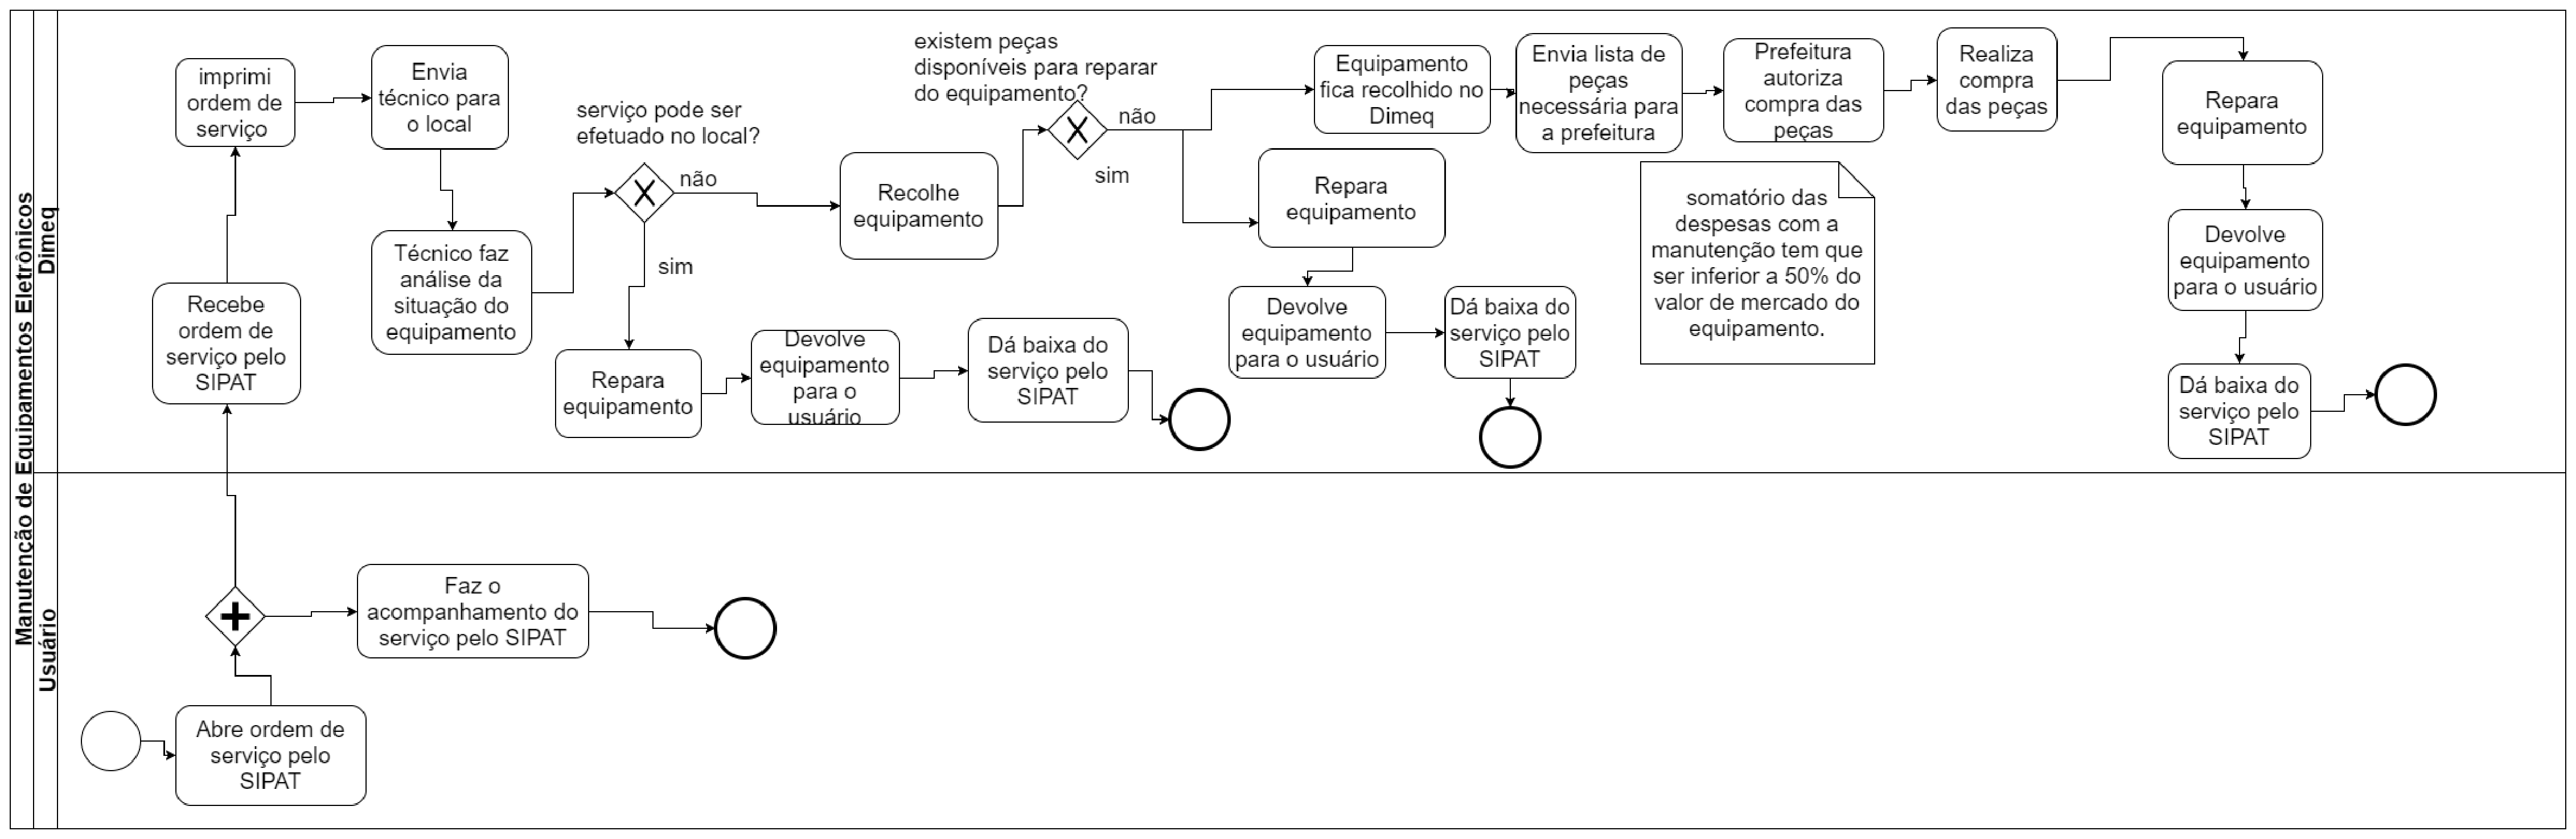
\includegraphics[width=1.5\textwidth]{processo_as_is}
\caption{Processo AS IS (atual) seguido pela DIMEQ. \textbf{Fonte: Autor.}}
\label{processo-as-is}
\end{figure}
\end{landscape} 

O processo foi desenhado a partir de entrevistas realizadas com um funcionário da Dimeq (Tabela~\ref{questionario}), e depois validado com o mesmo. Nas entrevistas foi possível perceber que existe um acompanhamento razoável do processo de manutenção, porém que está sujeito a diversas melhorias, que já são práticas comuns no mercado. Por exemplo, na entrevista foi perguntado ao técnico se eles sabem qual o custo total do reparo de um equipamento, contando as horas trabalhadas do técnico no reparo, as horas que o equipamento fica indisponível para o usuário, o que dependendo do equipamento, pode paralisar a atividade suportada por ele, o preço de peças que precisem ser compradas para que o reparo possa ser feito, a confiabilidade do equipamento quando ele passou por inúmeros reparos. A única forma de medição que eles tem segundo a entrevista é a de que se o valor da manutenção custar mais que 50\% do valor de um equipamento novo, eles o substituem, mas esse custo é apenas referente ao preço de um peça nova necessária. 
                                                                

\begin{table}[H]
\centering
\caption{Questionário repondido na entrevista com o funcionário da Dimeq. Fonte: Autor.}
\label{questionario}
\begin{tabular}{ |p{7cm}| p{8cm} |}
\hline
%\multicolumn{2}{|c|}{\textbf{Questionário Respondido na Entrevista}} \\ \hline
	Perguntas & Respostas \\ \hline
	Como são inventariados os equipamentos da Universidade de Brasília? & Pelo SIPAT. \\ \hline
	Como é feito o processo de manutenção? & Para iniciar o pedido de manutenção o usuário entra no SIPAT, descreve o problema, insere o tipo (reparo), depois o técnico vai ao local, se for possível ele realiza o reparo, senão, o equipamento é recolhido.Em seguida o equipamento é devolvido ao usuário. \\ \hline
	Quais são as áreas envolvidas no processo de manutenção? & Dimeq e prefeitura. \\ \hline
	Qual é o procedimento para se solicitar a manutenção de um equipamento? & A manutenção é solicitada pelo SIPAT. \\ \hline
	Este setor emprega algum método para saber a frequência de quebra de cada equipamento ou modelo de equipamento? Se existir, como é feito? & Pelo patrimônio (SIPAT) é possível saber quantas vezes o equipamento foi para a manutenção. \\ \hline
	É conhecido o valor gasto em cada manutenção prestada? & Não. \\ \hline
	É realizado algum tipo de manutenção preventiva? & Sim, existe uma seção de manutenção preventiva. \\ \hline
	Quem realiza o serviço de manutenção de equipamentos na Universidade? (Equipe interna? Algum prestador de serviço? A própria assistência técnica do fabricante?) & Se o equipamento estiver na garantia, a empresa fornecedora. Sem garantia, uma prestadora de serviço. \\ \hline
	Se a manutenção for interna, como são adquiridas as peças de reposição? São originais? Possuem garantia? & É feita uma lista de peças de reposição, contendo quais faltam, as mais usadas. Peças muito caras a UnB não libera recurso, usuário geralmente compra. O manual vai direto para o usuário. \\ \hline
	É dado algum prazo de garantia aos equipamentos que passaram por manutenção ? Se sim, qual? & Sim, 10 dias úteis.\\ \hline
\end{tabular}
\end{table}


Kardec e Nascif (2010) falam em Manutenção - Função Estratégica, que em empresas bem sucedidas o setor de manutenção tem reagido rapidamente a mudanças e esse posicionamento inclui uma crescente conscientização de quanto uma falha de equipamento afeta a segurança, da relação entre manutenção e qualidade do produto e de como as atividades realizadas nas empresas exigem cada vez mais uma maior disponibilidade e confiabilidade dos equipamentos, as mesmo tempo em que se busca diminuir os custos. Para se atingir essas características é necessário que todos os envolvidos no processo mudem suas atitudes. 

A Universidade de Brasília hoje possui quatro campi, sendo o central o Campus Darcy Ribeiro e os outros mais afastados são os da Ceilândia, Gama e Planaltina. Esse processo é seguido a risca, hoje, apenas no Darcy Ribeiro, pois devido a falta de técnicos (atualmente são apenas 10 técnicos para os quatro campi), os outros campi estão levando os equipamentos até o Darcy para que eles sejam reparados. Não existe a parte em que o técnico vai até o local, avalia a situação do equipamento. Pensando nisso, existem também vários riscos que podem ser considerados, como o transporte do equipamento de um local para o outro, que pode acarretar em maiores danos, o aumento no tempo de indisponibilização do equipamento para seu usuário, entre outros. 

Ao perguntar ao entrevistado, como eram realizadas as manutenções no campus do gama - FGA, ele disse que quem tem acesso ao SIPAT, para abrir as ordens de serviço é a secretaria do campus. Sendo que por falta de pessoal no Dimeq os equipamentos são levados até eles. 

A substituição dos equipamentos é feita após o Dimeq emitir um laudo técnico justificando a impossibilidade da recuperação do equipamento e a inviabilidade econômica. Após o laudo, o Centro de Custo deve requisitar a compra de um equipamento novo, seguindo os procedimento da Instrução Normativa SEDAP n. 205/1988.

Na entrevista, percebeu-se a necessidade de se ter um sistema mais completo, o qual dê maior suporte as atividades de manutenção, pois ele possui poucas funcionalidades direcionadas a manutenção, sendo elas de registro de ordem de serviço, acompanhamento do chamado, registro de quantas manutenções foram feitas no equipamento, mas sem ter uma análise mais detalhada sobre como essas informações possam gerar resultados significativos para instituição. Por isso, o trabalho busca formular indicadores que possam auxiliar aos usuários do sistema a tomar futuras decisões relacionadas a manutenção e substituição de equipamentos. \\*



